\documentclass[10pt]{beamer}

\usetheme[progressbar=frametitle]{metropolis}
\usepackage{appendixnumberbeamer}

\usepackage{booktabs}
\usepackage[scale=2]{ccicons}

\usepackage{pgfplots}
\usepgfplotslibrary{dateplot}

\usepackage{xspace}
\newcommand{\themename}{\textbf{\textsc{metropolis}}\xspace}

\title{236609 - MULTI ROBOT SYSTEMS}
\subtitle{Assignment 2 Presentation Template}% \date{\today}
\date{}

\date{}
\author{Netanel Ossi and Ben Hadad}
\institute{
The Taub Faculty of Computer Science\\
Technion - Israel Institute of Technology}

% \titlegraphic{\hfill\includegraphics[height=1.5cm]{logo.pdf}}

\begin{document}

\maketitle


\section{Single-Agent Dirt Collection}
\begin{frame}{Problem Description}
\textbf{Given:}

\begin{itemize}
    \item A start position of the robot
    \item A map of the room(as a matrix) 
\end{itemize}

\textbf{Do:}

\begin{itemize}
    \item cover great amount of areas in the room efficiently(without scanning same place twice, and fast as possible)
\end{itemize}
\end{frame}

\begin{frame}{Problem Description (continued)}
\begin{itemize}
    \item This problem is relevant to real world applications such as:  
    \begin{itemize}
    \item cleaning robots (for example, "Roomba")
\end{itemize}
\end{itemize}
\begin{figure}[t]
		\centering
		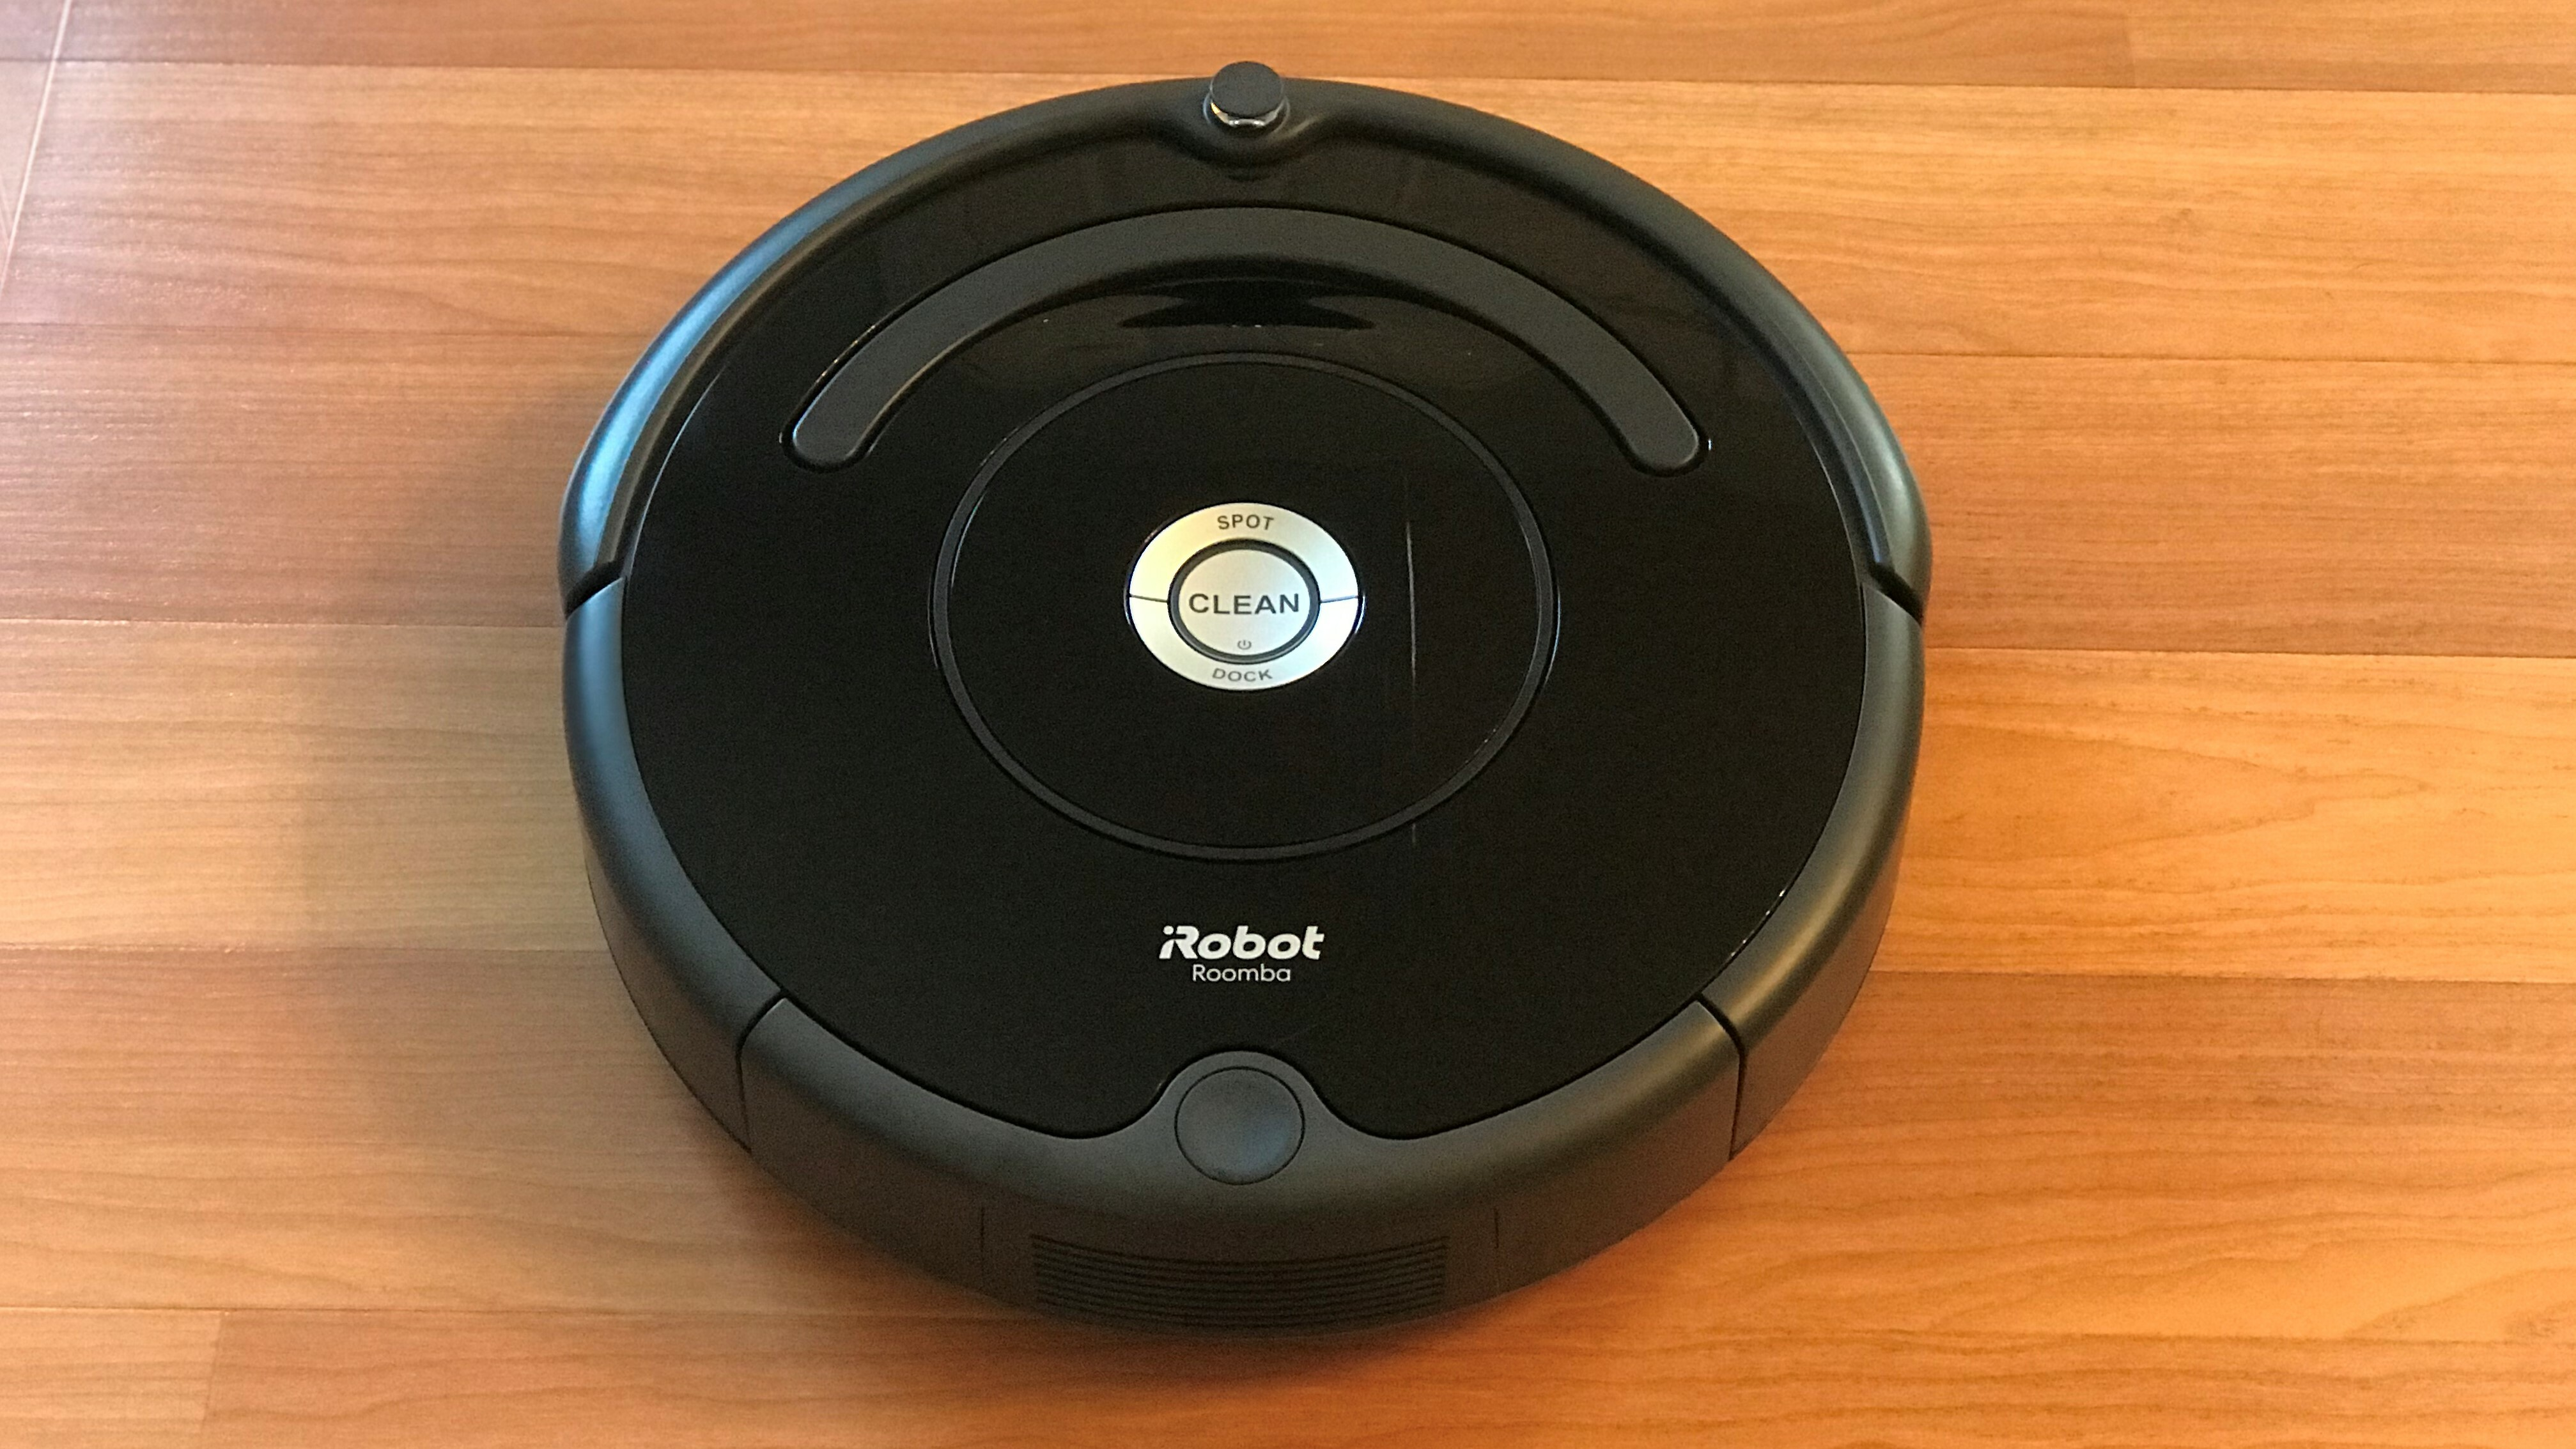
\includegraphics[width=0.3\textwidth]{images/roomba.jpg}
\end{figure}\hfill
\end{frame}

\begin{frame}{Problem Description (continued)}
\begin{itemize}
    \item This problem is hard because: 
    \begin{itemize}
    \item we have fixed amount of running time(4 mins), so we'll have to cover great amount of areas of the map as fast as possible
    \item the room map is unknown before executing
\end{itemize}
    \item An exhaustive approach to the solution would be:
    \begin{itemize}
    \item "plow field" moves, covering any point of the room
    \begin{figure}[t]
		\centering
		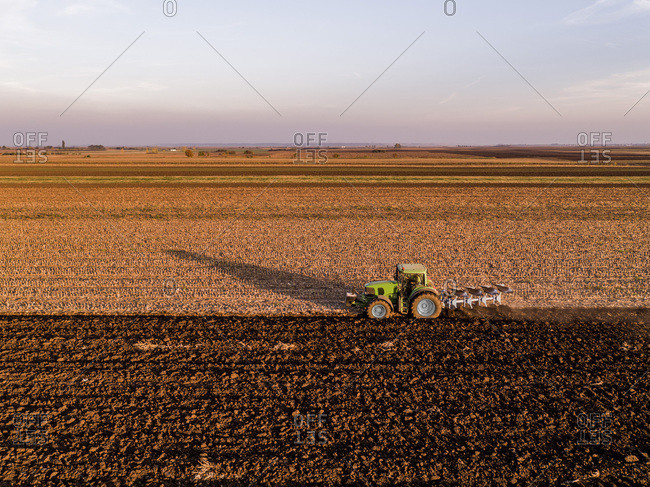
\includegraphics[width=0.3\textwidth]{images/plow.jpg}
    \end{figure}\hfill
\end{itemize}
\end{itemize}
\end{frame}


\begin{frame}{Model}

We {\bf model} the problem as a undirected weighted graph $G=(V, E)$ .first, we split the room into squares with a constant size. the nodes $V$ represent centers of the squares, and the edges $E$ represent the paths between the nodes.
the weight function is: 
\begin{itemize}
$w(v) = (w_1*dist_{from wall})*I_{Notvisited} $
\end{itemize}
where:
\begin{itemize}
% \begin{itemize}
%     \item {\bf dist_{from wall}:} {\bf the distance of the robot from the wall in the edge's direction}    
% \end{itemize}
\begin{itemize}
    \item {\bf $dist_{from wall}$:} { the distance of the robot from the wall in the node's direction}    
\end{itemize}
\begin{itemize}
    \item {\bf $I_{Notvisited} $:} { indicator, which is 1 if we haven't already visited the node, 0 otherwise}    
\end{itemize}
\end{itemize}
\end{frame}


\begin{frame}{Suggested Approach}

Our suggested solution takes as input the static map(as a matrix). we noticed that spiral movement saves time compared to moves with rotations, so we tried to find algorithm that has minimal number of rotations, to be efficient. when we'll get to a node, we'll make spiral moves, till we'll get close to a wall, and then move to the next node.
\end{frame}



 \begin{frame}{Implementation details}

 We implemented our approach using:
  \begin{itemize}
     \item \textbf{move algorithm:}
     given the robot's current position and step size, the algorithm calculates the heaviest edge that connected to the node, based on the weight function explained above. 
\end{itemize}
%  \end{frame}

% \begin{frame}{Implementation details(continued)}

    \begin{itemize}
         \item  \textbf{rotation algorithm:}
         when we get to a node, we'll make a spiral moves, till we'll get to a defined distance from a wall. and then we'll use the move algorithm, where "step size" is the max between the biggest spiral radius, and defined constant.  
    \end{itemize}
\end{frame}


\begin{frame}{Performance Guarantees}

\begin{itemize}
		\item Computational Efficiency 
		\item Generality
		\item Memory consumption
	\end{itemize}
	

\end{frame}



\begin{frame}{Details from the process}

\begin{itemize}
    \item The approach we presented was the third we tried. The first two failed because they weren't efficient under time limitation.
    \item Our approach can cover areas efficiently, but it cannot avoid obstacles and fails miserably if bump into obstacles while moving in spirals.
    \item Ideas for future development: finding the greatest area in the room, going to it's middle, making spiral moves around this dot, till getting close to a wall, and from there, move to the second largest area etc..
\end{itemize}

\end{frame}

\section{Single-agent inspection}

\begin{frame}{Problem Description}
\textbf{Given:}

\begin{itemize}
    \item A start position of the robot
    \item A static map of the room(as a matrix)
    \item A global cost-map of the room(as a matrix) 
\end{itemize}

\textbf{Find:}

\begin{itemize}
    \item the number of unmapped obstacles(spheres) estimated to exist in the room
\end{itemize}
\end{frame}

% \begin{figure}[t]
% 		\centering
% 		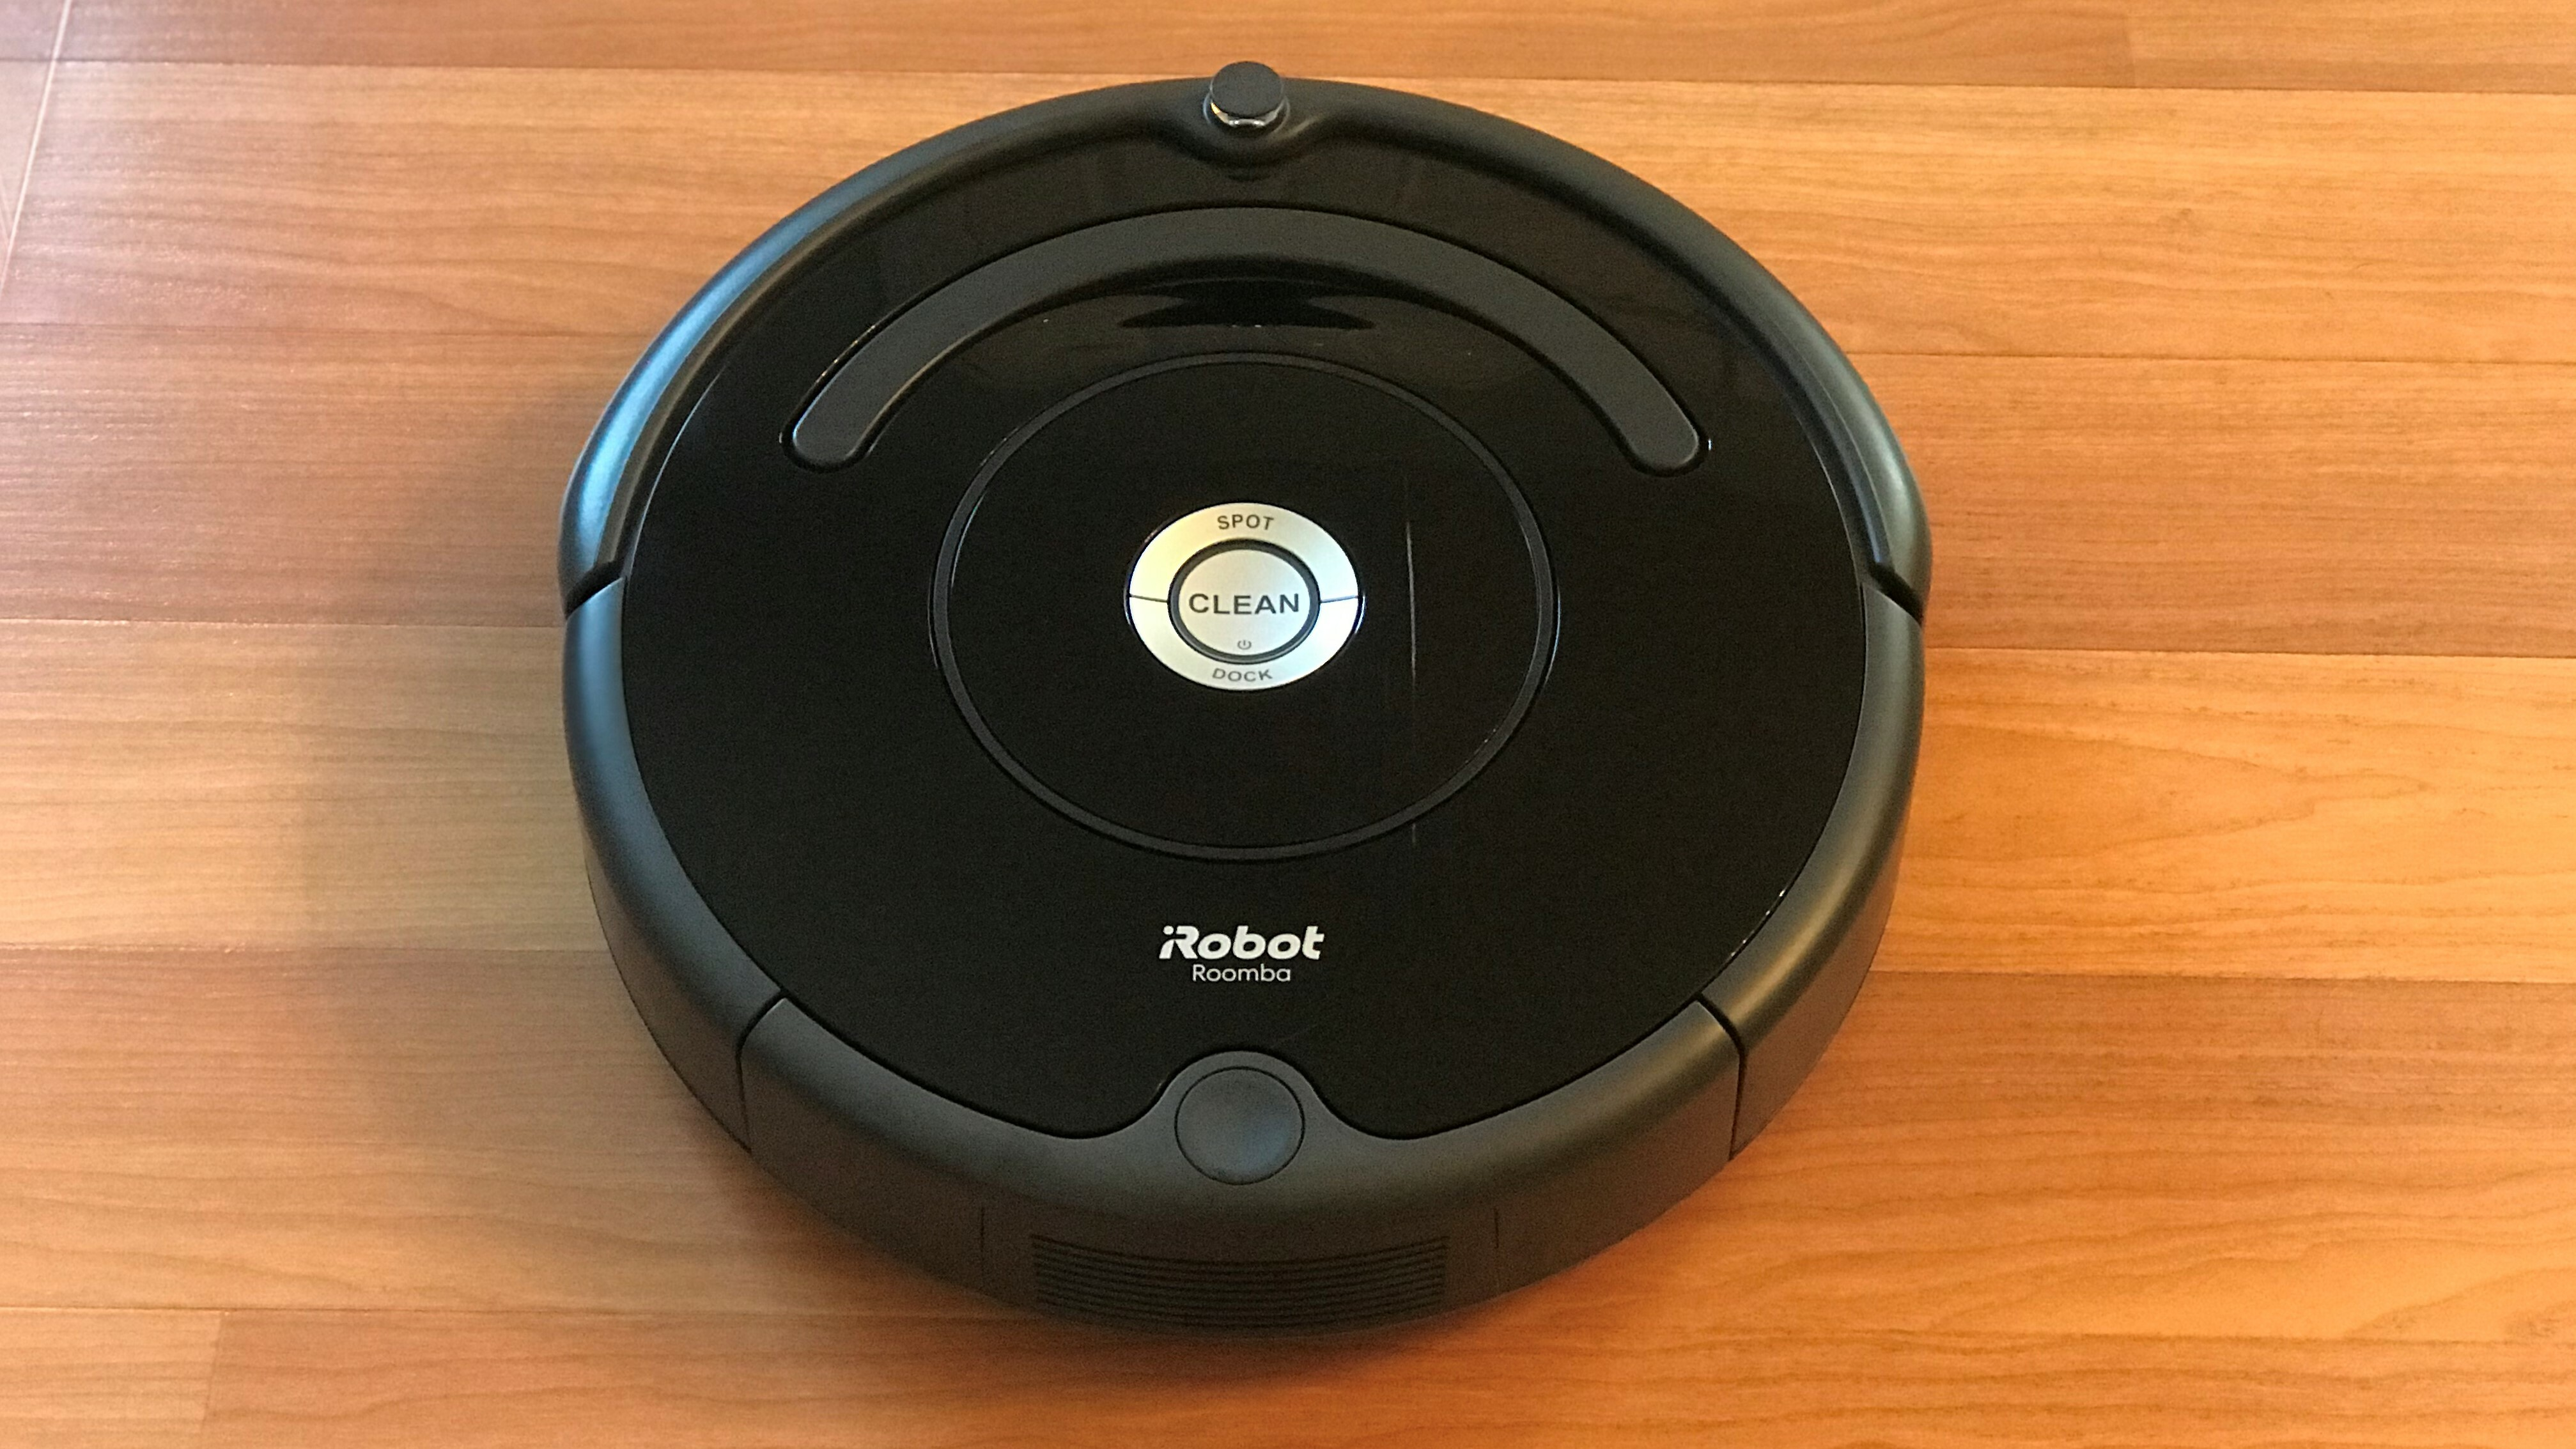
\includegraphics[width=0.3\textwidth]{images/roomba.jpg}
% 		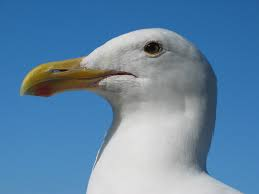
\includegraphics[width=0.3\textwidth]{images/example_image.jpg}
% \end{figure}\hfill
\begin{frame}{Problem Description (continued)}
\begin{itemize}
    \item This problem is relevant to real world applications such as:  
    \begin{itemize}
    \item Robocup Soccer League
    \item autonomous cars, have to detect unmapped obstacles in their area, and react to them
    \item cleaning robots need to detect and avoid obstacles
\end{itemize}
\end{itemize}
\begin{figure}[t]
		\centering
		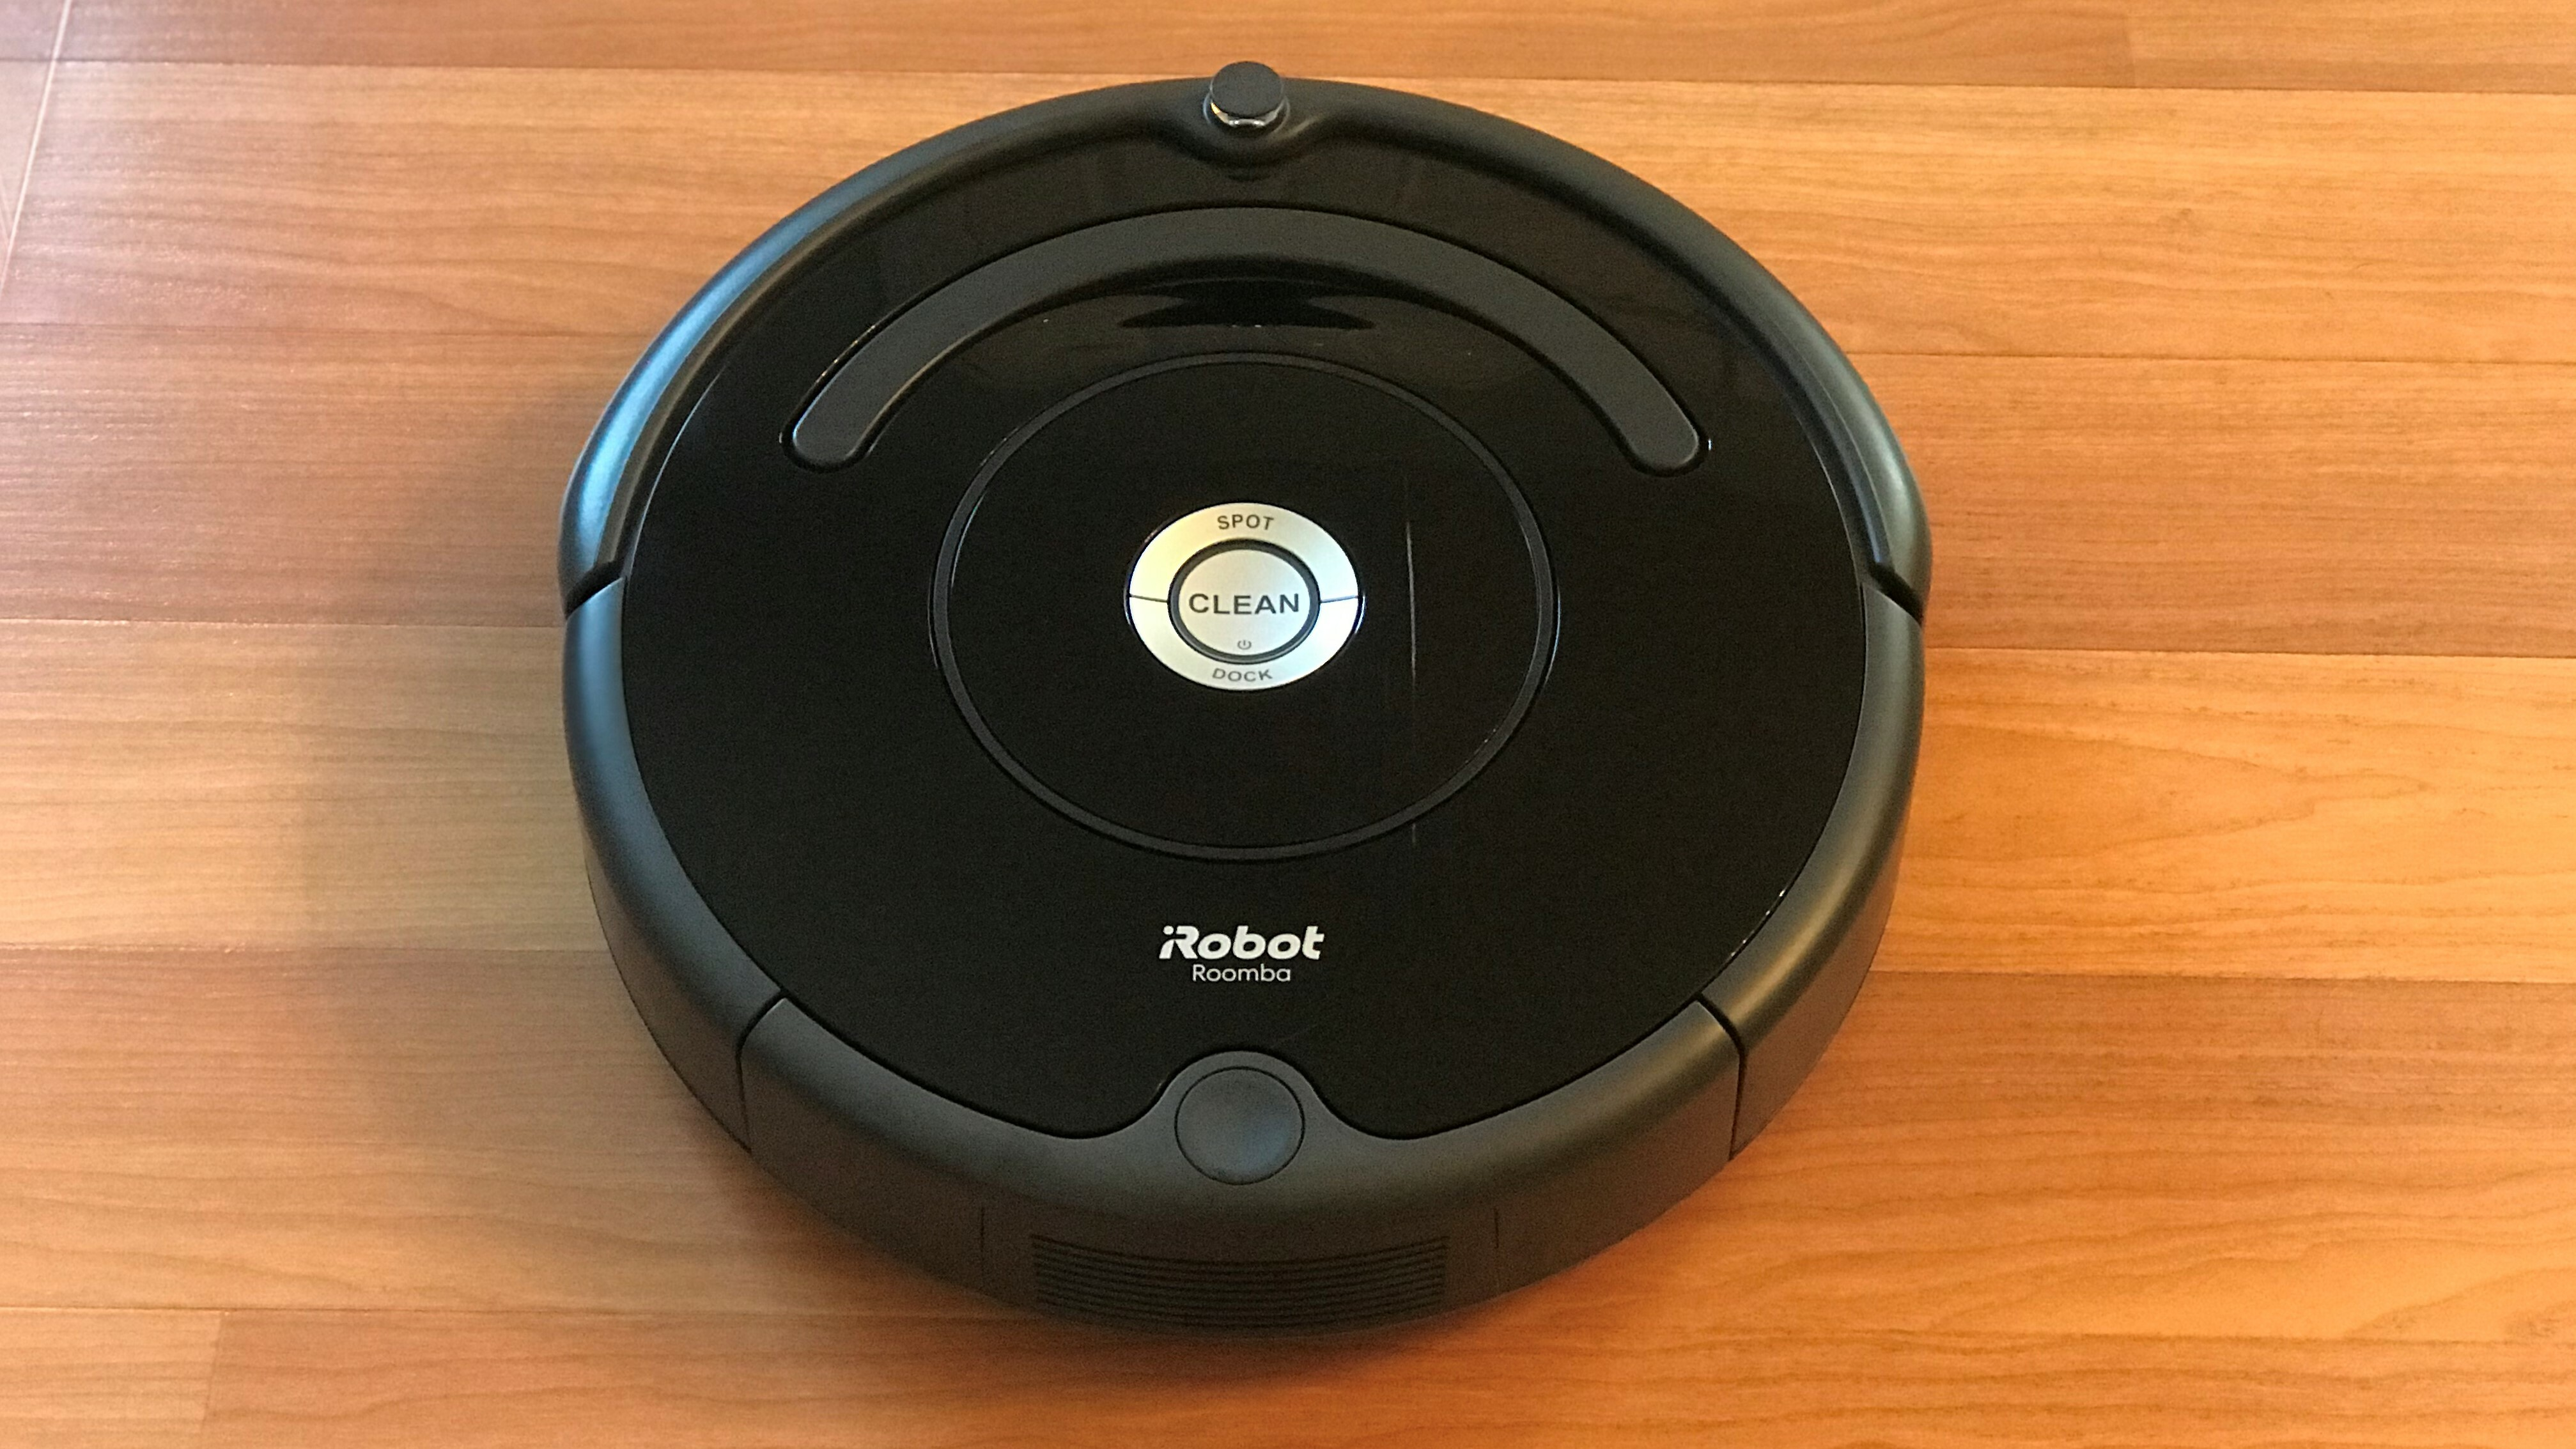
\includegraphics[width=0.3\textwidth]{images/roomba.jpg}
		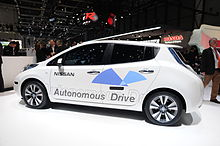
\includegraphics[width=0.3\textwidth]{images/car.jpg}
		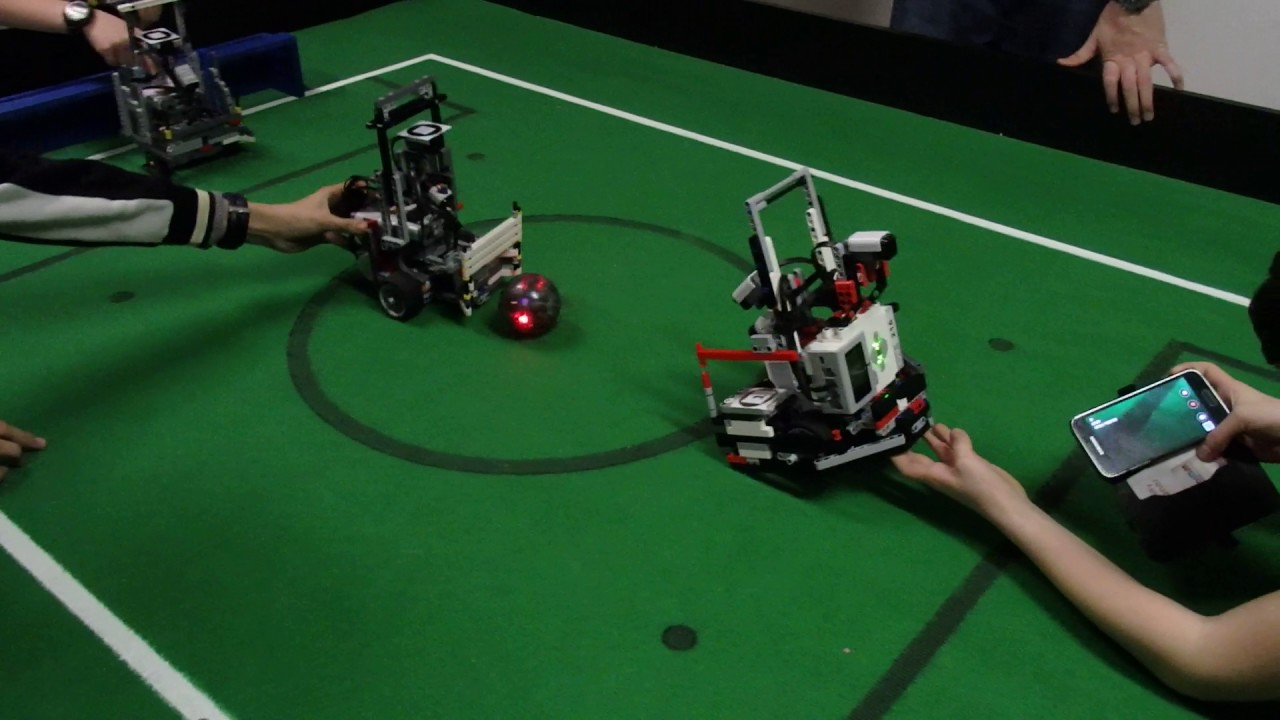
\includegraphics[width=0.3\textwidth]{images/soccer.jpg}
\end{figure}\hfill
\end{frame}

\begin{frame}{Problem Description (continued)}
\begin{itemize}
    \item This problem is hard because: 
    \begin{itemize}
    \item we have unknown amount of running time, so we'll have to scan big areas of the map efficiently(without scanning same place twice, and as fast as possible)
    \item the robot scan range is limited
    \item the room map is unknown before executing
     \item the spheres amount and locations are unknown
\end{itemize}
    \item An exhaustive approach to the solution would be:
    \begin{itemize}
    \item "plow field" moves(with width of scan range), scanning any point of the room
    \begin{figure}[t]
		\centering
		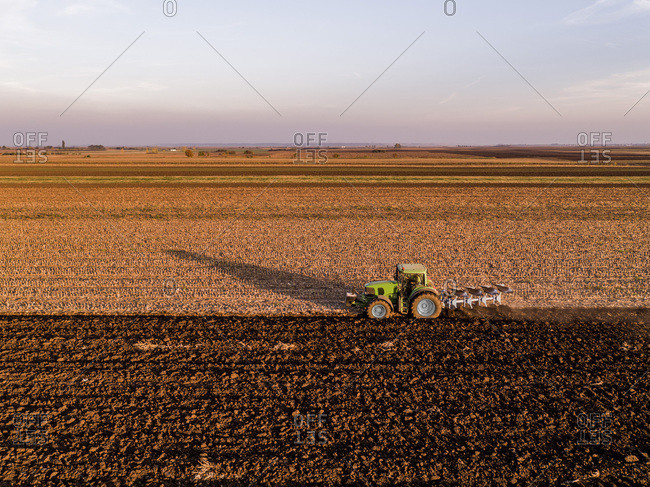
\includegraphics[width=0.3\textwidth]{images/plow.jpg}
    \end{figure}\hfill
\end{itemize}
\end{itemize}
\end{frame}

\begin{frame}{Model}

We {\bf model} the problem as a undirected weighted graph $G=(V, E)$. .first, we split the room into squares with a constant size(size of the scanning range). the nodes $V$ represent centers of the squares, and the edges $E$ represent the paths between the nodes.
the weight function is: 
\begin{itemize}
$w(v) = (w_1*dist_{from wall}+w_2*sphere_{exist})*I_{Notvisited} $
\end{itemize}
where:
\begin{itemize}
%     \item {\bf dist_{from wall}:} {\bf the distance of the robot from the wall in the edge's direction}    
% \end{itemize}
\begin{itemize}
    \item {\bf $dist_{from wall}$:} { the distance of the robot from the wall in the node's direction}    
\end{itemize}
\begin{itemize}
    \item {\bf $sphere_{exist}$ :} { the bigger area that a shpere takes from the node's square, the smaller the value.}
\end{itemize}
\begin{itemize}
    \item {\bf $I_{Notvisited} $:} { indicator, which is 1 if we haven't already visited the node, 0 otherwise}    
\end{itemize}
\end{itemize}
\end{frame}


\begin{frame}{Suggested Approach}

Our suggested solution takes as input the static map(as a matrix),global map(as a matrix) and the current position at the matrix. we noticed that for covering areas efficiently, we'll want to split the map into squares with constant size of the scanned range, and pass over areas that smaller than a sphere's size.
we also noticed that spheres have specific pattern in the cost map, and we'll be able to search for that pattern in order to identify spheres. also, we saw that when a robot is sent to a point inside a sphere, it gets stuck. so we'll have to make small moves, only in scanned areas.(like fog of war game:\url{https://en.wikipedia.org/wiki/Fog_of_war})

\begin{figure}[t]
		\centering
		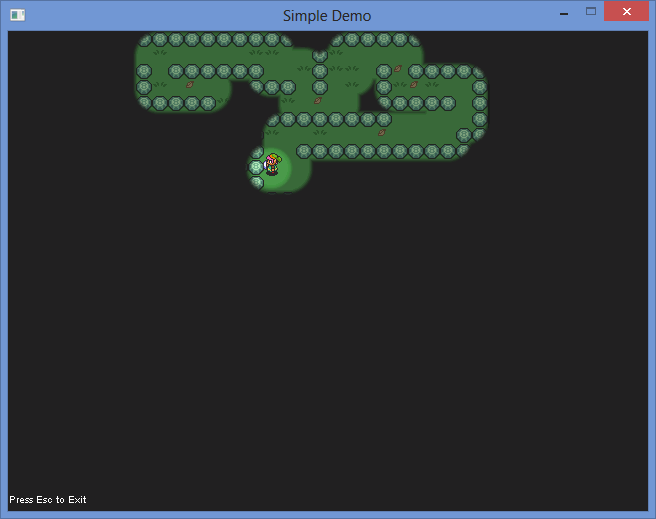
\includegraphics[width=0.2\textwidth]{images/fog.png}
    \end{figure}\hfill
\end{frame}



 \begin{frame}{Implementation details}

 We implemented our approach using:
  \begin{itemize}
     \item \textbf{move algorithm:}
     identical to the move algorithm from the cleaning problem. here step size is dynamic, taking into account the size of the scanned range, walls position and spheres that we already mapped.
         \item  \textbf{sphere detection algorithm:}
         when we arrive to a new square that we didn't scan, we'll examine the scanned area inside the updated global cost map, and search for a sphere pattern. If found, we'll calculate it's Estimated center, and add it to a list of centers.
\end{itemize}
 \end{frame}


\begin{frame}{Performance Guarantees}

\begin{itemize}
		\item Anytime 
		\item Computational Efficiency 
		\item Generality
		\item Memory consumption
	\end{itemize}
	

\end{frame}



\begin{frame}{Details from the process}

\begin{itemize}
    \item The approach we presented was the second we tried. The first failed because didn't take into account stepping on spheres.
    \item Our approach can identify spheres, while moving safely(only to scanned areas) it cannot detect spheres which the robot cannot scan(hidden behind another spheres, for example). our approach fails miserably if sphere size isn't known and identical for all spheres.
    \item Ideas for future development are being able to identify spheres while moving, without stopping at all, and without stepping on spheres.
\end{itemize}

\end{frame}



\end{document}
